\section{实验目的}
掌握 DBMS 提供的数据库用户和权限管理机制;理解存储过程概念,掌握存
储过程与触发器的使用;掌握数据库备份与恢复方法。

\section{实验预备内容}
\begin{enumerate}
  \item 阅读教材《数据库系统概论》相关章节。
  \item 阅读实验使用的数据库管理系统的相关帮助文档。
\end{enumerate}

\section{实验环境}
\begin{itemize}
  \item OS: Linux
  \item DBMS: OpenGauss DataBase
\end{itemize}

\section{实验内容}

\subsection{数据库安全性}
\begin{enumerate}
  \item 数据库账户的添加、删除
\begin{center}
\begin{minted}[xleftmargin=5mm,breaklines,breakanywhere]{sql}
-- 账户添加
CREATE USER JIM PASSWORD 'Bigdata@123';

-- 账户查看
SELECT * FROM pg_user;

-- 账户删除
DROP USER jim CASCADE;
\end{minted}
\end{center}
\begin{figure}[H]
  \begin{center}
    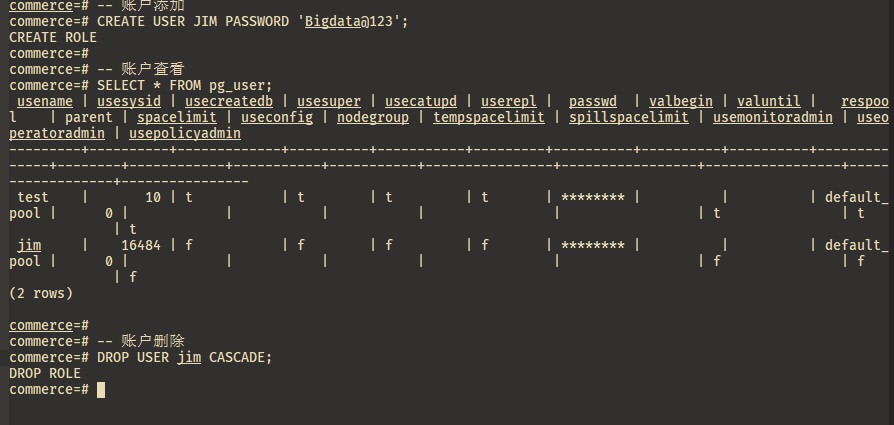
\includegraphics[width=0.95\textwidth]{./figures/account_management.jpg}
  \end{center}
  \caption{数据库账户的添加, 删除}
\end{figure}
  \item 对账户进行授予权限、收回权限。
\begin{center}
\begin{minted}[xleftmargin=5mm,breaklines,breakanywhere]{sql}
CREATE USER joe PASSWORD 'Bigdata@123';

-- 授予权限
 GRANT ALL PRIVILEGES TO joe;

-- 收回权限
REVOKE ALL PRIVILEGES FROM joe;
\end{minted}
\end{center}
\begin{figure}[H]
  \begin{center}
    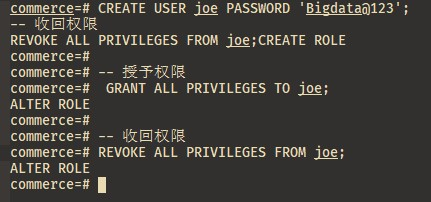
\includegraphics[width=0.95\textwidth]{./figures/account_perm.jpg}
  \end{center}
  \caption{对账户进行授予权限、收回权限}
\end{figure}
\end{enumerate}

\subsection{触发器,存储过程的使用}
\begin{enumerate}
  \item 创建存储过程并执行.
\begin{center}
\begin{minted}[xleftmargin=5mm,breaklines,breakanywhere]{sql}
CREATE TABLE t_test(c1 INT, c2 INT);

-- 创建存储过程
CREATE OR REPLACE procedure insert_data
IS
a INT;
b INT;
BEGIN
a=1;
b=2;
INSERT INTO t_test VALUES(a,b);
INSERT INTO t_test VALUES(b,a);
END;
/

-- 执行存储过程
CALL insert_data();
SELECT * FROM t_test;
\end{minted}
\end{center}
\begin{figure}[H]
  \begin{center}
    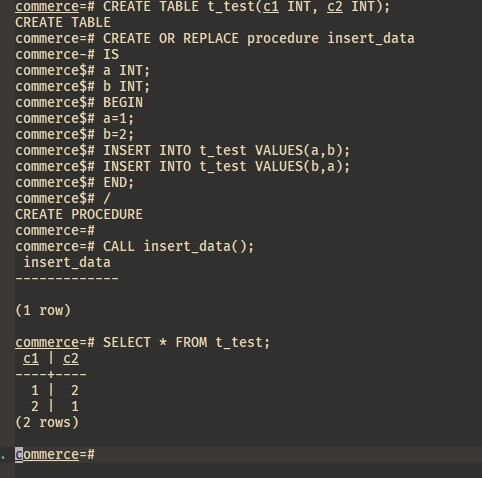
\includegraphics[width=0.95\textwidth]{./figures/procedure.jpg}
  \end{center}
  \caption{创建存储过程并执行}
\end{figure}
  \item 创建触发器并测试效果。
\begin{center}
\begin{minted}[xleftmargin=5mm,breaklines,breakanywhere]{sql}
--创建源表及触发表
CREATE TABLE test_trigger_src_tbl(id1 INT, id2 INT, id3 INT);
CREATE TABLE test_trigger_des_tbl(id1 INT, id2 INT, id3 INT);

--创建触发器函数
CREATE OR REPLACE FUNCTION tri_insert_func() RETURNS TRIGGER AS
  $$
  DECLARE
  BEGIN
    INSERT INTO test_trigger_des_tbl VALUES(NEW.id1, NEW.id2, NEW.id3);
    RETURN NEW;
  END
  $$ LANGUAGE PLPGSQL;

CREATE OR REPLACE FUNCTION tri_update_func() RETURNS TRIGGER AS
  $$
  DECLARE
  BEGIN
    UPDATE test_trigger_des_tbl SET id3 = NEW.id3 WHERE id1=OLD.id1;
    RETURN OLD;
  END
  $$ LANGUAGE PLPGSQL;

CREATE OR REPLACE FUNCTION TRI_DELETE_FUNC() RETURNS TRIGGER AS
  $$
  DECLARE
  BEGIN
          DELETE FROM test_trigger_des_tbl WHERE id1=OLD.id1;
          RETURN OLD;
  END
  $$ LANGUAGE PLPGSQL;

-- 创建INSERT触发器
CREATE TRIGGER insert_trigger
  BEFORE INSERT ON test_trigger_src_tbl
  FOR EACH ROW
  EXECUTE PROCEDURE tri_insert_func();

-- 创建UPDATE触发器
CREATE TRIGGER update_trigger
  AFTER UPDATE ON test_trigger_src_tbl
  FOR EACH ROW
  EXECUTE PROCEDURE tri_update_func();

-- 创建DELETE触发器
CREATE TRIGGER delete_trigger
  BEFORE DELETE ON test_trigger_src_tbl
  FOR EACH ROW
  EXECUTE PROCEDURE tri_delete_func();

-- 执行INSERT触发事件并检查触发结果
INSERT INTO test_trigger_src_tbl VALUES(100,200,300);
SELECT * FROM test_trigger_src_tbl;
SELECT * FROM test_trigger_des_tbl;

-- 执行UPDATE触发事件并检查触发结果
UPDATE test_trigger_src_tbl SET id3=400 WHERE id1=100;
SELECT * FROM test_trigger_src_tbl;
SELECT * FROM test_trigger_des_tbl;

-- 执行DELETE触发事件并检查触发结果
DELETE FROM test_trigger_src_tbl WHERE id1=100;
SELECT * FROM test_trigger_src_tbl;
SELECT * FROM test_trigger_des_tbl;

-- 修改触发器
ALTER TRIGGER delete_trigger ON test_trigger_src_tbl RENAME TO delete_trigger_renamed;

-- 禁用insert_trigger触发器
ALTER TABLE test_trigger_src_tbl DISABLE TRIGGER insert_trigger;

-- 禁用当前表上所有触发器
ALTER TABLE test_trigger_src_tbl DISABLE TRIGGER ALL;

--删除触发器
DROP TRIGGER insert_trigger ON test_trigger_src_tbl;
DROP TRIGGER update_trigger ON test_trigger_src_tbl;
DROP TRIGGER delete_trigger_renamed ON test_trigger_src_tbl;
\end{minted}
\end{center}
\begin{figure}[H]
  \begin{center}
    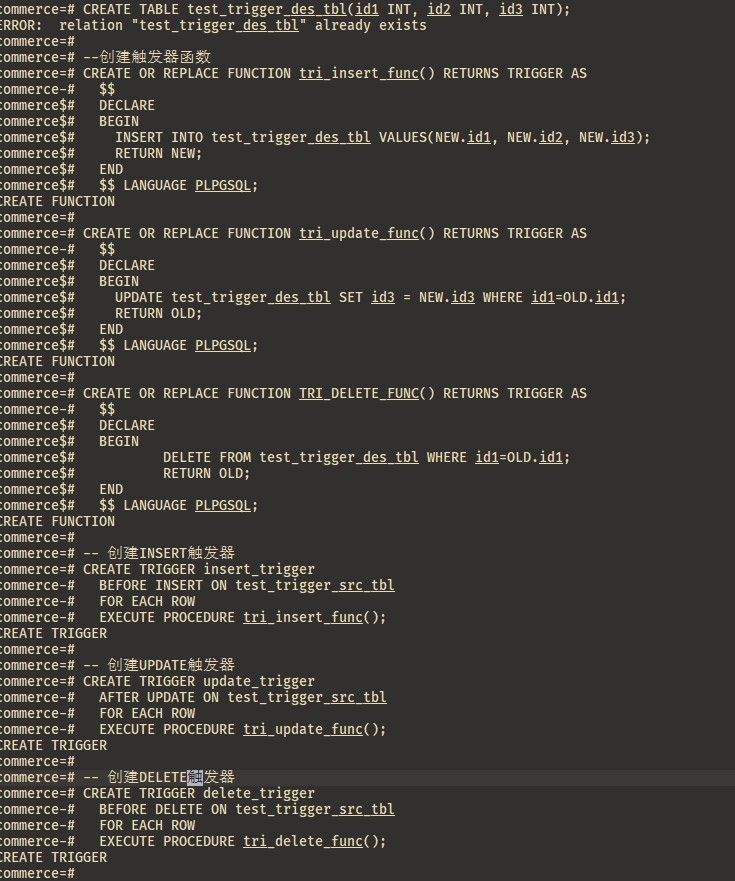
\includegraphics[width=0.95\textwidth]{./figures/trigger0.jpg}
  \end{center}
  \caption{创建触发器并测试效果}
\end{figure}
\begin{figure}[H]
  \begin{center}
    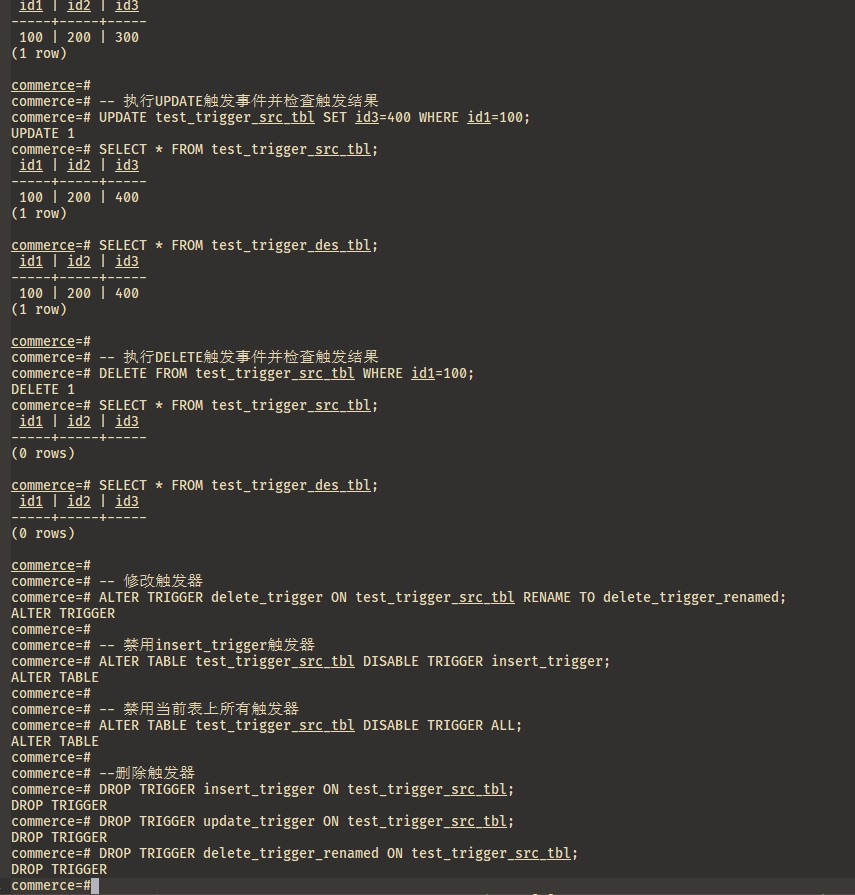
\includegraphics[width=0.95\textwidth]{./figures/trigger1.jpg}
  \end{center}
  \caption{创建触发器并测试效果}
\end{figure}
\end{enumerate}

\subsection{数据库备份与恢复}
\begin{enumerate}
  \item 对所创建的数据库进行备份
\begin{center}
\begin{minted}[xleftmargin=5mm,breaklines,breakanywhere]{sql}
DROP TABLE IF EXISTS customer_t1;
CREATE TABLE customer_t1
(
 c_customer_sk integer,
 c_customer_id char(5),
 c_first_name char(6),
 c_last_name char(8)
);
INSERT INTO customer_t1 (c_customer_sk, c_customer_id, c_first_name) VALUES
(3769, 'hello', DEFAULT) ,
(6885, 'maps', 'Joes'),
(4321, 'tpcds', 'Lily'),
(9527, 'world', 'James');

DROP TABLE IF EXISTS customer_t2;
CREATE TABLE customer_t2
(
 c_customer_sk integer,
 c_customer_id char(5),
 c_first_name char(6),
 c_last_name char(8)
);
INSERT INTO customer_t2 (c_customer_sk, c_customer_id, c_first_name) VALUES
(3769, 'hello', DEFAULT) ,
(6885, 'maps', 'Joes'),
(9527, 'world', 'James');

DROP user IF EXISTS lucy;
CREATE USER lucy WITH PASSWORD "Bigdata@123";
\c - lucy
DROP TABLE IF EXISTS lucy.mytable;
CREATE TABLE mytable (firstcol int);
INSERT INTO mytable values (100);
\end{minted}
\end{center}
\begin{center}
\begin{minted}[xleftmargin=5mm,breaklines,breakanywhere]{bash}
mkdir -p /home/test/physical/backup
gs_basebackup -D /home/test/physical/backup -p 26000
\end{minted}
\end{center}
\begin{figure}[H]
  \begin{center}
    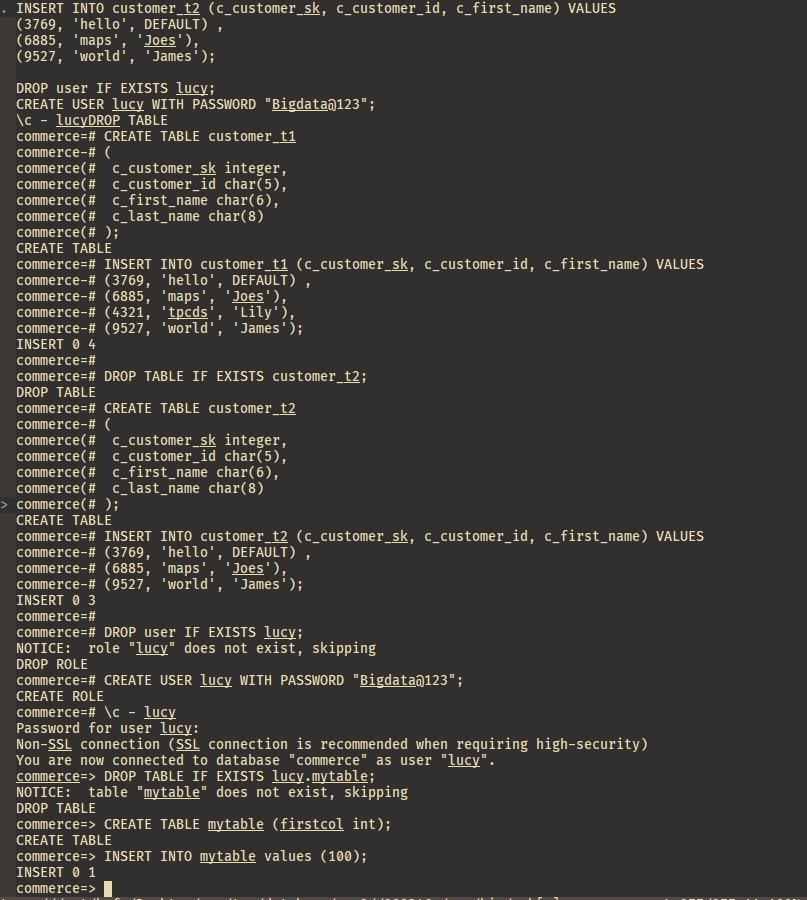
\includegraphics[width=0.95\textwidth]{./figures/backup.jpg}
  \end{center}
  \caption{对所创建的数据库进行备份}
\end{figure}
\begin{figure}[H]
  \begin{center}
    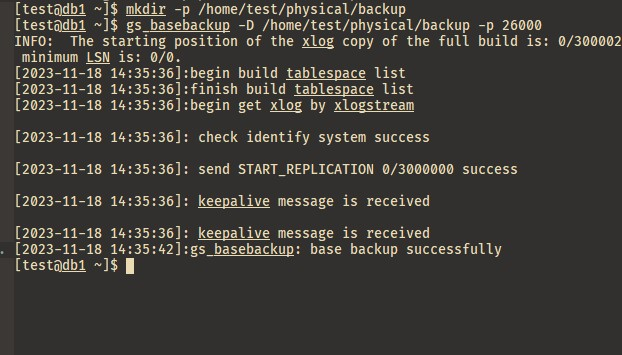
\includegraphics[width=0.95\textwidth]{./figures/backup1.jpg}
  \end{center}
  \caption{对所创建的数据库进行备份}
\end{figure}
  \item 利用备份进行数据库恢复
\begin{minted}[xleftmargin=5mm,breaklines,breakanywhere]{bash}
gs_om -t stop
cd /gaussdb/data/db1
rm -rf *
cp -r /home/test/physical/backup/. /gaussdb/data/db1
gs_om -t start
\end{minted}
\begin{figure}[H]
  \begin{center}
    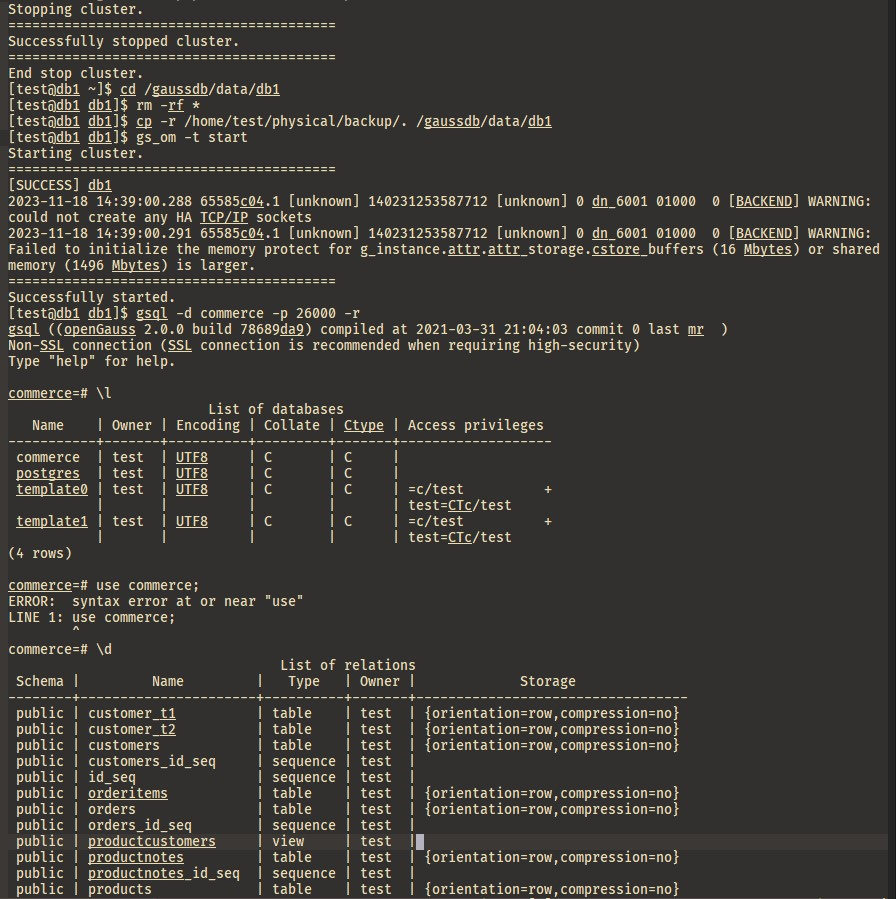
\includegraphics[width=0.95\textwidth]{./figures/restore.jpg}
  \end{center}
  \caption{利用备份进行数据库恢复}
\end{figure}
\end{enumerate}

\section{实验总结}

\subsection{实验涉及到的相关知识}
\begin{itemize}
  \item 数据库账户的添加和删除;
  \item 对账户进行授予权限, 收回权限;
  \item 创建并执行存储过程;
  \item 创建触发器并测试效果;
  \item 删除触发器;
  \item 数据库的备份和恢复.
\end{itemize}

\subsection{实验遇到的问题及其解决}
没有问题.
